\chapter{Introduction}
\label{ch:intro}
\pagenumbering{arabic}

The increasing popularity and the intensive usage of computational systems in the everyday of modern life creates the need for easier and less invasive forms of user recognition. While enter a hard to memorize password in a terminal and identify a person placing a human to listen to telephone calls are the status quo for respectively authentication and identification, voice biometrics presents itself as a continuing improvement alternative. Passwords can be forgotten and people are biased and unable to be massive trained, but the unique characteristics of a person's voice combined with an automatic speaker recognizer (ASR) outperform any ``manual" attempt.

Speech is the most natural way humans have to communicate, being incredibly complex and with numerous specific details related to its producer, \refbib{Bimbot et. al.}{bimbot.et.al.2004}. Therefore, it is expected an increasing usage of vocal interfaces to perform actions such as computer login, voice search (e.g., Apple Siri, Google Now and Samsung S Voice) and identification of speakers in a conversation and its content. At present, fingerprint biometrics is adopted in several solutions (e.g., ATMs, \refbib{Wang \& Wu}{wang.wu.2002}), authentication through facial recognition comes as built-in software for average computers and iris scan was adopted for a short time by United Kingdom and permanently by United Arab Emirates border controls, \refbib{Sasse}{sasse.2007}, \refbib{Raisi \& Khouri}{raisi.khouri.2008}. These examples indicate a near future where biometrics are common, with people talking to the computer and receiving concise answers, and cash withdrawals allowed via a combination of speaker verification, corrected captcha dictated and other techniques.

Current commercial products based on voice technology (e.g., Dragon Naturally Speaking, KIVOX and VeriSpeak) are usually intended to perform either \textbf{speech recognition} (\emph{what} is being said) or \textbf{speaker recognition} (\emph{who} is speaking). Voice search applications are designed to determine the content of a speech, usually with no concern about who the speaker is or if there is more than one, while computer login and telephone fraud prevention supplement a memorized personal identification code with speaker verification, \refbib{Reynolds}{reynolds.1995a}, not interested on the message spoken. Few applications perform both processes, such as automatic speaker labeling of recorded meetings, that transcribes what each person is saying. To achieve this goal, numerous voice processing techniques have become known in industry and academy, e.g., Natural Language Processing (NLP), Hidden Markov Models (HMMs) and Gaussian Mixture Models (GMMs). Although all of these are interesting state-of-the-art techniques, the subject covered by this paper is the area of speaker recognition and only a small subset of these techniques will be unraveled.

\section{Speaker Recognition}
\label{sec:speaker-recognition}

As stated in \refbib{Reynolds \& Campbell}{reynolds.campbell.2008}, speaker recognition may be divided in two subareas. The first is \textbf{speaker identification}, aimed to determine the identity of a speaker from a non-unitary set of known speakers. This task is also named speaker identification in \textbf{closed set}. In the second, \textbf{speaker verification}, the goal is to determine if a speaker is who he or she claims to be, not an imposter. As the set of imposters is unknown, this is an \textbf{open set} problem. An intermediate task is \textbf{open set identification}, when an ``unmatched class" is added in order to categorize all unknown speakers.

\begin{figure}[ht]
    \centering
    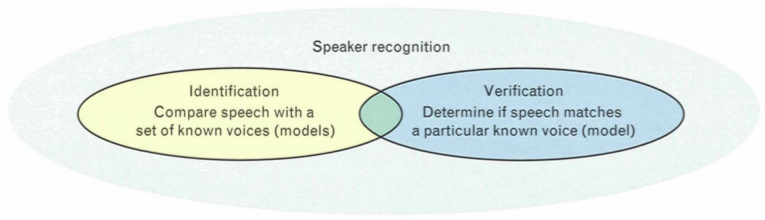
\includegraphics[width=\textwidth]{speaker-recognition}
    \caption{Speaker identification and speaker verification are different, but not entirely, \refbib{Reynolds}{reynolds.1995a}.}
    \label{fig:speaker-recognition}
\end{figure}

The text used may be constrained, such as by type (e.g., digits and letters) and/or by number of words used (e.g., one word or sentences). In \textbf{text-dependent} systems the content of the speech is relevant to the evaluation, and the testing texts must belong to the training set (not necessarily be the entire set), \refbib{Hébert}{hebert.2008}. A change in the training text demands an complete new training section. \textbf{Text-independent} systems have no restrictions to the message in both sets, with the non-textual characteristics of the user's voice (e.g., pitch and accent) being the important aspects to the evaluator. These characteristics are presented in different sentences, usage of foreign languages and even gibberish. Between the extremes in constraints falls the \textbf{vocabulary-dependent system}, which constrains the speech to come from a limited vocabulary (e.g., digits) from which test words or phrases are selected (e.g., ``two" or ``one-two-three"), \refbib{Reynolds}{reynolds.1995a}.

The focus of this paper is in \textbf{text-independent speaker recognition} and to achieve that, Gaussian Mixture Models are used.

\section{Objectives}

The objectives of this study is to implement an ASR that executes the listed actions:

\begin{itemize}\itemsep0pt
    \item From a group of enrolled speakers identify who produced a given speech signal, for all speakers in the group;
    \item Determine if a speaker is the claimed enrolled speaker or an imposter, given the speech signal produced. This experiment is performed for a group of enrolled speakers and for a group of imposters.
    \item Analyze the performance for different number of mixtures and features.
\end{itemize}

\section{Document Structure}

\chapterref{speaker-recognition-system} contains basic information about speaker recognition, as well as the basic architecture of speaker identification and verification systems. The feature extraction process is explained in \chapterref{feature-extraction}, from the reasons for its use to the chosen technique (Mel-Frequency Cepstral Coefficient, MFCC). In \chapterref{gmm} the GMM and the Universal Background Model (UBM) are detailed. Experiments are described in \chapterref{experiments}, as well as its results. Finally, \chapterref{conclusion} concludes the study.